% ============================================================
%  TERM PROJECT – PROPOSAL
%  Databases · THGA Bochum
% ============================================================
\documentclass[11pt,a4paper]{article}

\usepackage{thga-db}
\usepackage{caption}
\usepackage{tikz}
\usetikzlibrary{arrows.meta,positioning}

\renewcommand{\thgaKurs}{Databases}
\renewcommand{\thgaDatum}{Summer Term 2026}
\newcommand{\authorName}{Mohamed Yassine Hachimi}
\newcommand{\projectTitle}{HandwerkerKasse -- Material and Invoice Tracker with Profit Analysis per Job}
\begin{document}
\thispagestyle{empty}
\thgaTitel{Term Project – Proposal}{\projectTitle}

\begin{infobox}
\textbf{Author:} \authorName \\
\textbf{Module:} Introduction to Database Management Systems · THGA Bochum \\
\textbf{Submitted to:} Stephan Bökelmann · \href{mailto:sboekelmann@ep1.rub.de}{sboekelmann@ep1.rub.de} \\
\textbf{Target size:} about 6 pages
\end{infobox}

% ============================================================
\section{Application domain and motivation}
% ============================================================

HandwerkerKasse is a database-driven web application for small craft businesses.
The system allows users to manage customers, jobs, materials and invoices.
The main goal is to provide a clear overview of job profitability by comparing
the invoice amount with the used material costs.

The application is designed for local craft businesses, self-employed workers
and small service providers. It helps users track projects, record used
materials, create invoices and identify whether a job was profitable. A typical usage scenario is an electrician creating a new customer order,
adding required materials such as cables and components, and generating an
invoice after completing the work. The system then calculates the estimated
profit by subtracting material costs from the invoice amount.

% ============================================================
\section{Data model -- ER sketch}
% ============================================================

\begin{figure}[ht]
  \centering
  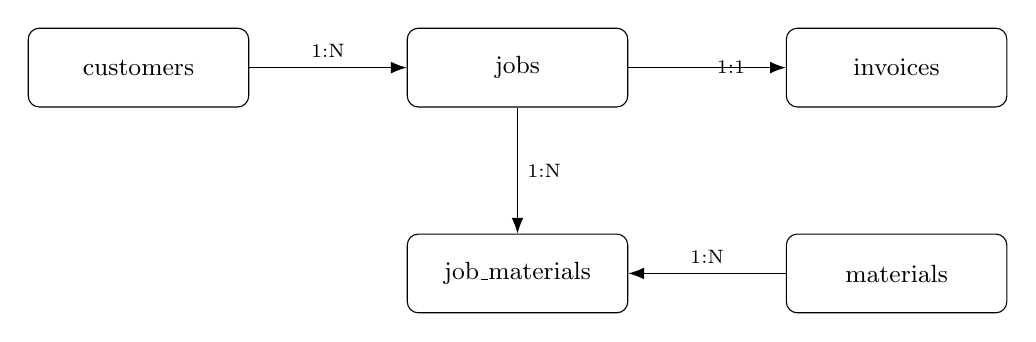
\begin{tikzpicture}[
    box/.style={draw, rounded corners, minimum width=2.8cm, minimum height=1cm, align=center, font=\small},
    node distance=1.6cm and 2cm
  ]
    \node[box] (customers) {customers};
    \node[box, right=of customers] (jobs) {jobs};
    \node[box, below=of jobs] (jobmat) {job\_materials};
    \node[box, right=of jobmat] (materials) {materials};
    \node[box, above=of materials] (invoices) {invoices};

    \draw[-{Latex[length=2mm]}] (customers) -- node[above,font=\scriptsize]{1:N} (jobs);
    \draw[-{Latex[length=2mm]}] (jobs) -- node[right,font=\scriptsize]{1:N} (jobmat);
    \draw[-{Latex[length=2mm]}] (materials) -- node[above,font=\scriptsize]{1:N} (jobmat);
    \draw[-{Latex[length=2mm]}] (jobs) -- node[right,font=\scriptsize]{1:1} (invoices);
  \end{tikzpicture}
  \caption{ER sketch of the handcraft business data model}
  \label{fig:er}
\end{figure}

Figure~\ref{fig:er} shows the ER model of the HandwerkerKasse system.
The main entities are customers, jobs, materials and invoices.
A customer can have multiple jobs, while each job can contain multiple
materials. The N:M relationship between jobs and materials is represented by
the \texttt{job\_materials} table, which also stores the quantity of each used material.
Each job can have one related invoice containing the billing information.

% ============================================================
\section{From model to schema}
% ============================================================

The relational schema consists of the following tables:

\begin{itemize}
  \item \texttt{customers}(\underline{id}, name, email, phone)
  \item \texttt{jobs}(\underline{id}, 
        \emph{customer\_id}, title, status, date)
  \item \texttt{materials}(\underline{id}, name, purchase\_price)
  \item \texttt{job\_materials}(\underline{id},
        \emph{job\_id}, \emph{material\_id}, quantity)
  \item \texttt{invoices}(\underline{id},
        \emph{job\_id}, amount, payment\_status)
\end{itemize}

\textbf{Normalisation.} The database schema follows the principles of the third normal form (3NF).
Each table stores one specific type of information and relationships are
represented using foreign keys instead of duplicated data.

% ============================================================
\section{API design}
% ============================================================

The FastAPI backend provides RESTful CRUD endpoints for all main entities.
The API acts as the communication layer between the frontend application and
the PostgreSQL database.

The frontend communicates with the backend using HTTP requests and JSON data.
Read operations are provided through GET requests, while write operations
require a valid \texttt{X-API-Key} header.

The profitability calculation is implemented using SQL JOIN operations between
\texttt{jobs}, \texttt{job\_materials}, \texttt{materials} and
\texttt{invoices}. Aggregation is used to calculate the total material costs
for each job.

\renewcommand{\arraystretch}{1.2}
\begin{tabularx}{\linewidth}{@{}p{2cm}p{4cm}X@{}}
\toprule
\textbf{Method} & \textbf{Path} & \textbf{Purpose} \\
\midrule

\texttt{GET} &
\texttt{/customers} &
Returns all customers. \\

\texttt{POST} &
\texttt{/customers} &
Creates a new customer. Requires X-API-Key. \\

\texttt{GET} &
\texttt{/jobs} &
Returns all jobs. \\

\texttt{POST} &
\texttt{/jobs} &
Creates a new job. Requires X-API-Key. \\

\texttt{PUT} &
\texttt{/jobs/\{id\}} &
Updates an existing job. Requires X-API-Key. \\

\texttt{DELETE} &
\texttt{/jobs/\{id\}} &
Deletes an existing job. Requires X-API-Key. \\

\texttt{GET} &
\texttt{/materials} &
Returns all available materials. \\

\texttt{POST} &
\texttt{/materials} &
Creates a new material entry. Requires X-API-Key. \\

\texttt{POST} &
\texttt{/job\_materials} &
Assigns materials and quantities to a job.
Requires X-API-Key. \\

\texttt{GET} &
\texttt{/invoices} &
Returns all invoices. \\

\texttt{POST} &
\texttt{/invoices} &
Creates a new invoice. Requires X-API-Key. \\

\texttt{GET} &
\texttt{/jobs/profit} &
Returns jobs with calculated profit values using JOIN
and aggregation. \\

\bottomrule
\end{tabularx}

\textbf{Profit calculation.}

The endpoint \texttt{GET /jobs/profit} calculates the estimated profit of
each job using the following formula:

\[
\text{Profit} =
\text{Invoice Amount}
-
\sum(\text{Quantity} \times \text{Purchase Price})
\]

The calculation combines invoice data with material usage data. The result
contains the invoice amount, total material costs and the calculated profit
for every job.

\textbf{Example response:}

\begin{verbatim}
GET /jobs/profit

[
 {
  "job_id": 1,
  "title": "Electrical installation",
  "invoice_amount": 1200,
  "material_cost": 350,
  "profit": 850
 }
]
\end{verbatim}

Unauthorized write requests without a valid
\texttt{X-API-Key} are rejected by the backend with an HTTP 401/403 response.
% ============================================================
\section{Frontend prototype (wireframes)}
% ============================================================

The frontend is a lightweight desktop application installed as a Debian
package (.deb). At startup it asks for the API URL and X-API-Key.
The application provides screens for customers, jobs, materials and invoices.

The main screen displays a list of jobs and their profitability.
Forms allow users to create and update records through the FastAPI endpoints.

\begin{figure}[ht]
\centering
\begin{minipage}[t]{0.47\linewidth}\centering
  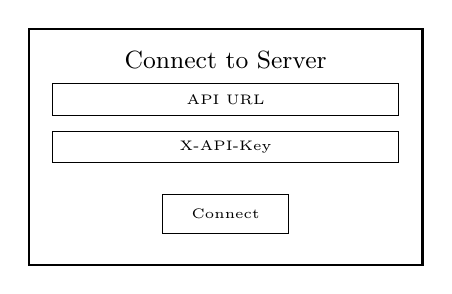
\begin{tikzpicture}
    \draw[thick] (0,0) rectangle (5,3);
    \node[font=\small] at (2.5,2.6) {Connect to Server};
    \draw (0.3,1.9) rectangle (4.7,2.3); \node[font=\tiny] at (2.5,2.1){API URL};
    \draw (0.3,1.3) rectangle (4.7,1.7); \node[font=\tiny] at (2.5,1.5){X-API-Key};
    \draw (1.7,0.4) rectangle (3.3,0.9); \node[font=\tiny] at (2.5,0.65){Connect};
  \end{tikzpicture}
  \captionof{figure}{Startup connection dialog: API URL + X-API-Key.}
  \label{fig:fe-connect}
\end{minipage}\hfill
\begin{minipage}[t]{0.47\linewidth}\centering
  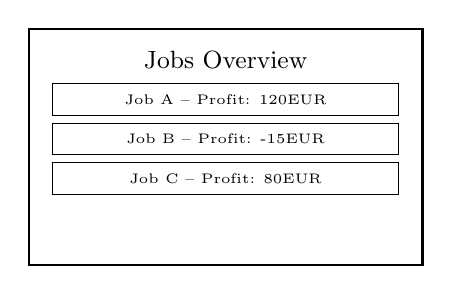
\begin{tikzpicture}
    \draw[thick] (0,0) rectangle (5,3);
    \node[font=\small] at (2.5,2.6) {Jobs Overview};
    \draw (0.3,1.9) rectangle (4.7,2.3); \node[font=\tiny] at (2.5,2.1){Job A -- Profit: 120EUR};
    \draw (0.3,1.4) rectangle (4.7,1.8); \node[font=\tiny] at (2.5,1.6){Job B -- Profit: -15EUR};
    \draw (0.3,0.9) rectangle (4.7,1.3); \node[font=\tiny] at (2.5,1.1){Job C -- Profit: 80EUR};
  \end{tikzpicture}
  \captionof{figure}{Main screen: job list with calculated profit, calls \texttt{GET /jobs/profit}.}
  \label{fig:fe-main}
\end{minipage}

\vspace{1em}

\begin{minipage}[t]{0.47\linewidth}\centering
  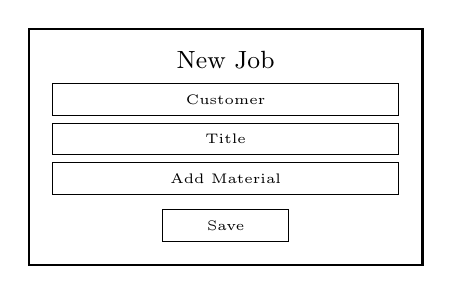
\begin{tikzpicture}
    \draw[thick] (0,0) rectangle (5,3);
    \node[font=\small] at (2.5,2.6) {New Job};
    \draw (0.3,1.9) rectangle (4.7,2.3); \node[font=\tiny] at (2.5,2.1){Customer};
    \draw (0.3,1.4) rectangle (4.7,1.8); \node[font=\tiny] at (2.5,1.6){Title};
    \draw (0.3,0.9) rectangle (4.7,1.3); \node[font=\tiny] at (2.5,1.1){Add Material};
    \draw (1.7,0.3) rectangle (3.3,0.7); \node[font=\tiny] at (2.5,0.5){Save};
  \end{tikzpicture}
  \captionof{figure}{Detail form: add job and materials, calls \texttt{POST /jobs} and \texttt{POST /job\_materials}.}
  \label{fig:fe-detail}
\end{minipage}\hfill
\begin{minipage}[t]{0.47\linewidth}\centering
  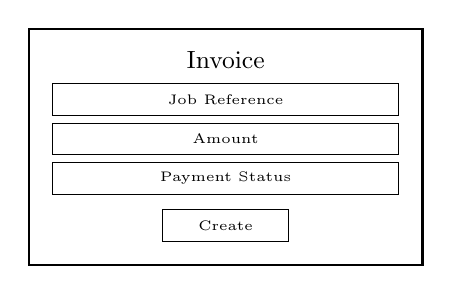
\begin{tikzpicture}
    \draw[thick] (0,0) rectangle (5,3);
    \node[font=\small] at (2.5,2.6) {Invoice};
    \draw (0.3,1.9) rectangle (4.7,2.3); \node[font=\tiny] at (2.5,2.1){Job Reference};
    \draw (0.3,1.4) rectangle (4.7,1.8); \node[font=\tiny] at (2.5,1.6){Amount};
    \draw (0.3,0.9) rectangle (4.7,1.3); \node[font=\tiny] at (2.5,1.1){Payment Status};
    \draw (1.7,0.3) rectangle (3.3,0.7); \node[font=\tiny] at (2.5,0.5){Create};
  \end{tikzpicture}
  \captionof{figure}{Invoice screen: create and view invoices per job, calls \texttt{POST /invoices} and \texttt{GET /invoices}.}
  \label{fig:fe-second}
\end{minipage}
\end{figure}

Figures~\ref{fig:fe-connect}--\ref{fig:fe-second} show the four screens of the
prototype. Figure~\ref{fig:fe-connect} shows the connection dialog that
collects the API URL and X-API-Key at startup; Figure~\ref{fig:fe-main}
shows the main screen listing all jobs together with their calculated profit,
reading from \texttt{GET /jobs/profit}; Figure~\ref{fig:fe-detail} shows the
form used to add a new job and assign materials to it, calling
\texttt{POST /jobs} and \texttt{POST /job\_materials}; and
Figure~\ref{fig:fe-second} shows the invoice screen, where an invoice is
created for a completed job via \texttt{POST /invoices}.

% ============================================================
\section{Operation with Docker Compose}
% ============================================================

The backend is deployed using Docker Compose.
The docker-compose.yml file contains two main services:
a PostgreSQL database service and a FastAPI backend service.

Database credentials and configuration values are stored in an .env file.
The backend container communicates with PostgreSQL through the internal Docker
network. The complete backend deployment runs on the lecture server.

% ============================================================
\section{Scope, milestones and risks}
% ============================================================

\textbf{Scope.} The project contains five database tables and approximately 15 FastAPI endpoints covering CRUD operations.

\textbf{Milestones and schedule.}

\renewcommand{\arraystretch}{1.2}
\begin{tabularx}{\linewidth}{@{}p{1.4cm}Xp{1.8cm}@{}}
\toprule
\textbf{Week} & \textbf{Milestone} & \textbf{Est. hours} \\
\midrule
1 & Database schema, ER model and seed data ready & 8 \\
2--3 & FastAPI CRUD endpoints with X-API-Key protection & 12 \\
4--5 & Frontend implementation and .deb packaging & 10 \\
6 & Testing, documentation and video preparation & 10 \\
\bottomrule
\end{tabularx}

\textbf{Risks.} Two risks were identified for this project. First, the profit
calculation depends on complete and correct material price data; missing or
outdated purchase prices in the \texttt{materials} table would lead to an
incorrect profitability report. Second, the .deb packaging and
frontend-backend integration could take longer than planned if dependency or
configuration issues arise on the lecture server, which would put pressure on
the remaining schedule.

% ============================================================
\section{Acceptance criteria and testing}
% ============================================================

This section states when the system counts as done and correct, and how this
is proven. Each criterion is formulated as a checkable statement, followed by
the test that backs it. The risk named above is covered by a dedicated test
case.

\textbf{Acceptance criteria.}
\begin{itemize}[topsep=2pt]
  \item A job or invoice that violates a constraint (e.g. missing
        \texttt{customer\_id} or a negative amount) is rejected by the API
        (returns 4xx).
  \item \texttt{GET /jobs/profit} returns the correct profit value for each
        job, calculated as invoice amount minus the summed cost of all
        associated materials (JOIN + aggregation).
  \item Write endpoints (\texttt{POST /jobs}, \texttt{POST /job\_materials},
        \texttt{POST /invoices}) without a valid X-API-Key are refused
        (401/403).
\end{itemize}

\textbf{Test plan.}
\begin{itemize}[topsep=2pt]
  \item \textbf{Database:} verify PRIMARY KEY constraints on all id columns,
        FOREIGN KEY constraints between \texttt{jobs}--\texttt{customers},
        \texttt{job\_materials}--\texttt{jobs},
        \texttt{job\_materials}--\texttt{materials} and
        \texttt{invoices}--\texttt{jobs}, and NOT NULL constraints on
        required fields such as customer name and invoice amount.
  \item \textbf{API:} endpoint tests covering the happy path and error cases
        (e.g. missing fields, invalid IDs, missing API key) using
        \texttt{pytest} and FastAPI's \texttt{TestClient} against a test
        database.
  \item \textbf{Business rule:} a dedicated test inserts a job with known
        material costs and invoice amount, then checks that
        \texttt{GET /jobs/profit} returns the expected profit value,
        covering the risk of incorrect price data named above.
\end{itemize}

\vspace{1em}
\begin{infobox}
\textbf{Effort budget:} the whole term project (system, documentation and video)
should fit into roughly \textbf{40\,h of work} over at most \textbf{2 months}.
Keep your scope within that budget.
\end{infobox}

\end{document}